\newpage
\section{Simulation Analysis}
\label{sec:simulation}
This section covers circuit simulation in ngspice, where the output voltage gain, the lower and upper cutoff frequencies and the input and output impedances were measured. However, in order to calculate the output impedance of the whole circuit, a different circuit had to be used. In this circuit the voltage source $V_in$ and the resistance $R_in$ were replaced by a short circuit and the load $R_L$ was replaced by a voltage source $V_o$.

In the following table gain, the cutoff frequencies, the bandwidth, the input and output impedances and the cost and merit of the circuit are presented. Furthermore, the graphs also show the frequency response of the output voltage gain and input and output impedances.

\begin{table}[h!]
  \centering
  \begin{tabular}{|c|c|}
    \hline    
    {\bf Name} & {\bf Value} \\ \hline
    gain & 6.059407e+01\\ \hline
lower & 8.155929e+00\\ \hline
upper & 2.178859e+06\\ \hline
bandwidth & 2.178851e+06\\ \hline
zin & 1.215084e+03\\ \hline
cost & 5.916600e+03\\ \hline
merit & 2.735974e+03\\ \hline

    @gb[i] & 0.000000e+00\\ \hline
@r1[i] & 0.000000e+00\\ \hline
@r2[i] & 0.000000e+00\\ \hline
@r3[i] & 0.000000e+00\\ \hline
@r4[i] & 0.000000e+00\\ \hline
@r5[i] & -2.85235e-03\\ \hline
@r6[i] & 0.000000e+00\\ \hline
@r7[i] & 0.000000e+00\\ \hline
v(1) & 0.000000e+00\\ \hline
v(2) & 0.000000e+00\\ \hline
v(3) & 0.000000e+00\\ \hline
v(5) & 0.000000e+00\\ \hline
v(6) & 8.671785e+00\\ \hline
v(7) & 0.000000e+00\\ \hline
v(8) & 0.000000e+00\\ \hline
v(9) & 0.000000e+00\\ \hline

  \end{tabular}
 \caption{Measured values (gain, cutoff frequencies, bandwidth, input and output impedances and the cost and merit of the circuit).}
  \label{tab:optabs}
\end{table}

\begin{figure}[h!] \centering
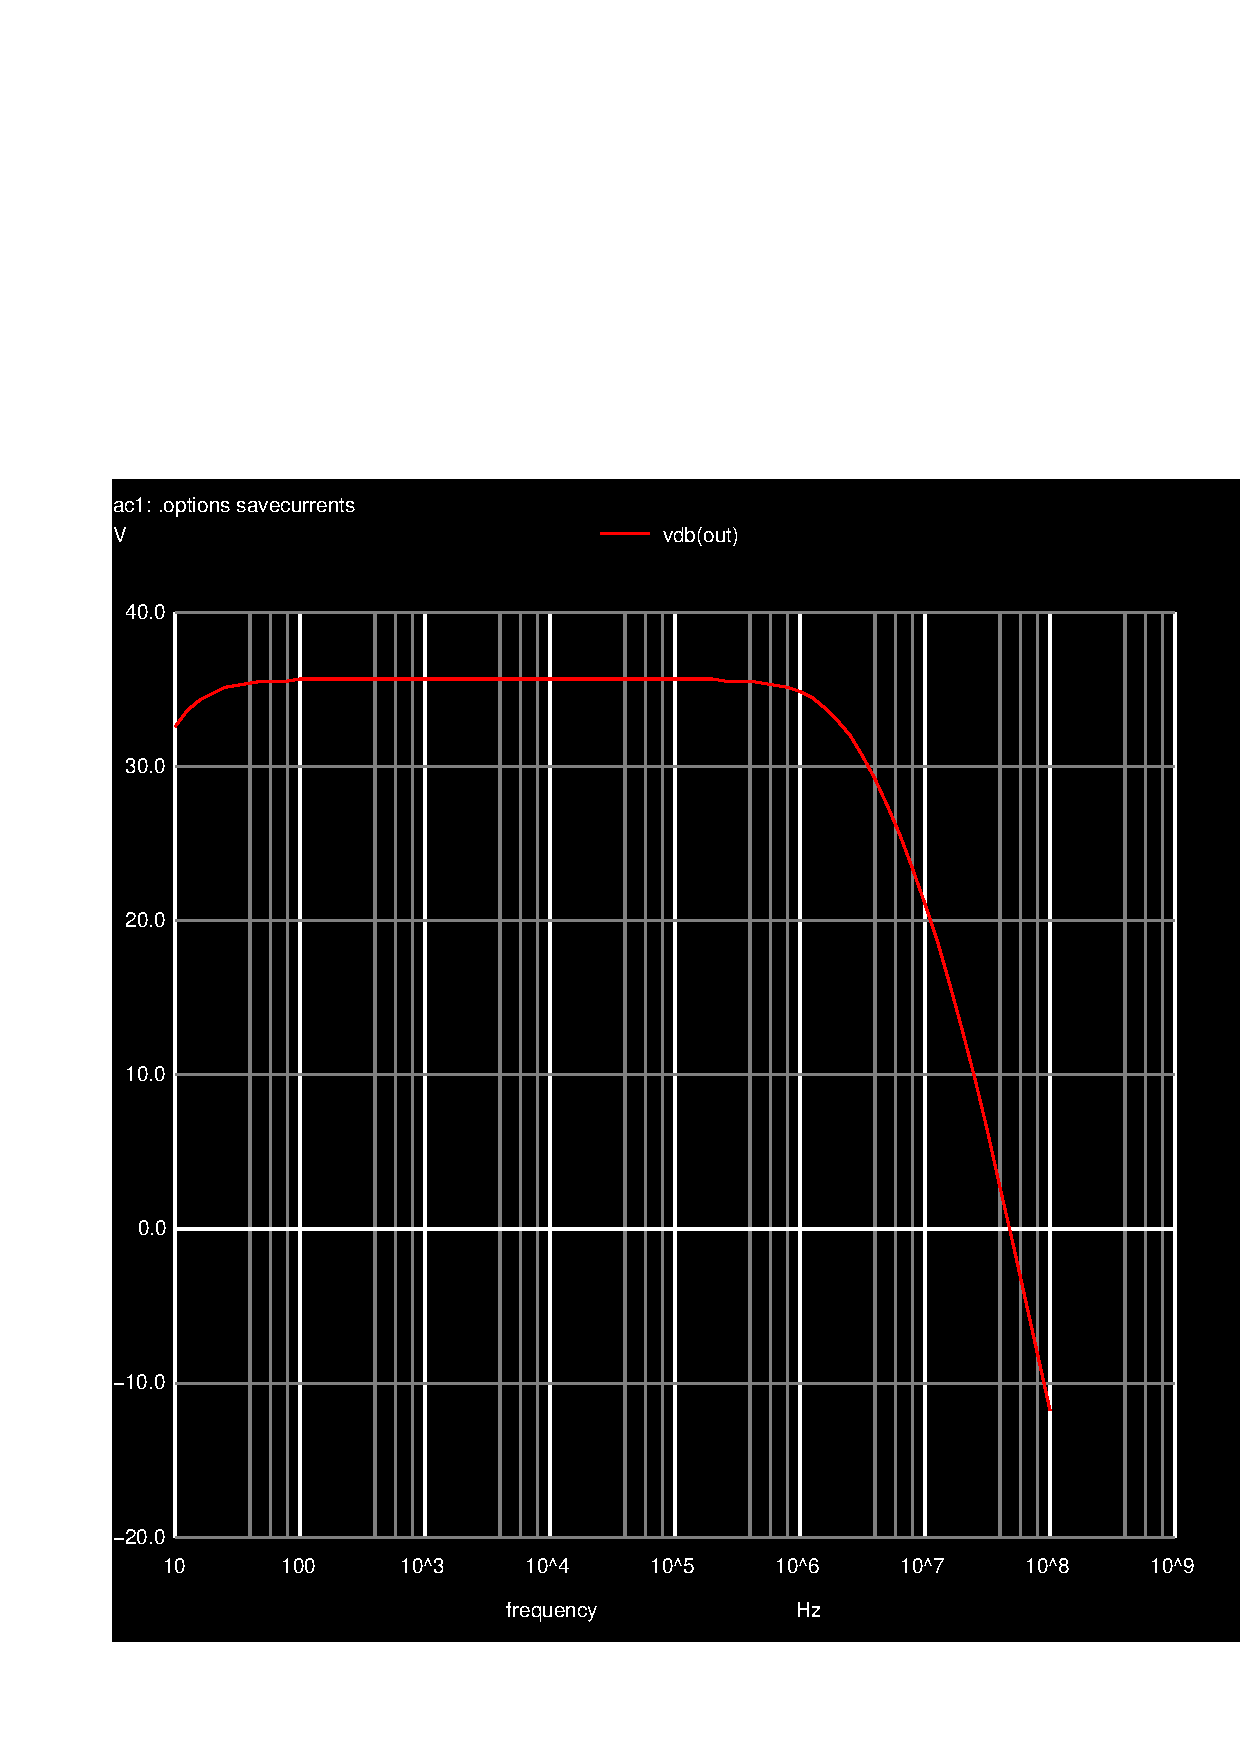
\includegraphics[width=7.5cm]{../sim/vo2f.pdf}
\caption{Frequency response of the output voltage gain in the passband.}
\label{fig:output voltage gain}
\end{figure}

\begin{figure}[h!] \centering
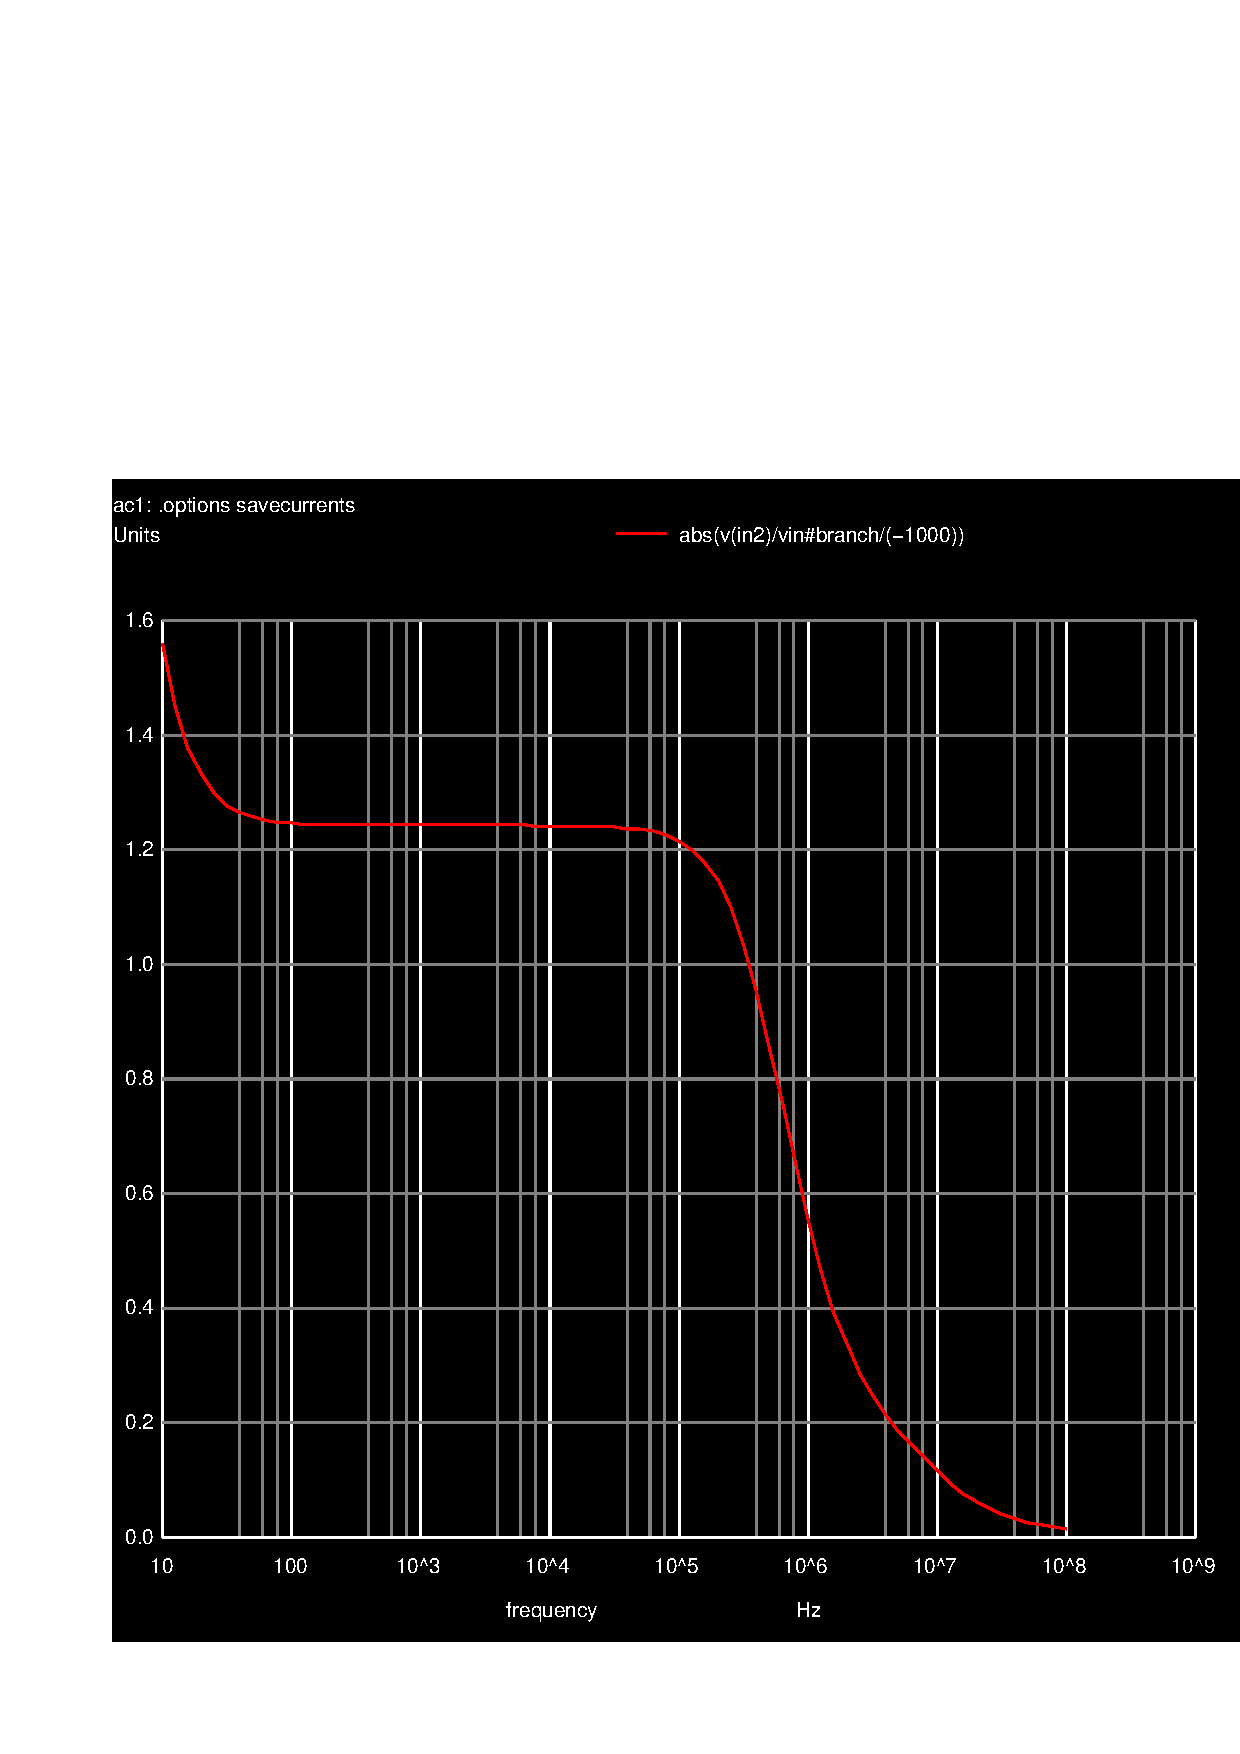
\includegraphics[width=7.5cm]{../sim/zin.pdf}
\caption{Frequency response of the input impedance of the circuit.}
\label{fig:input impedance}
\end{figure}

\begin{figure}[h!] \centering
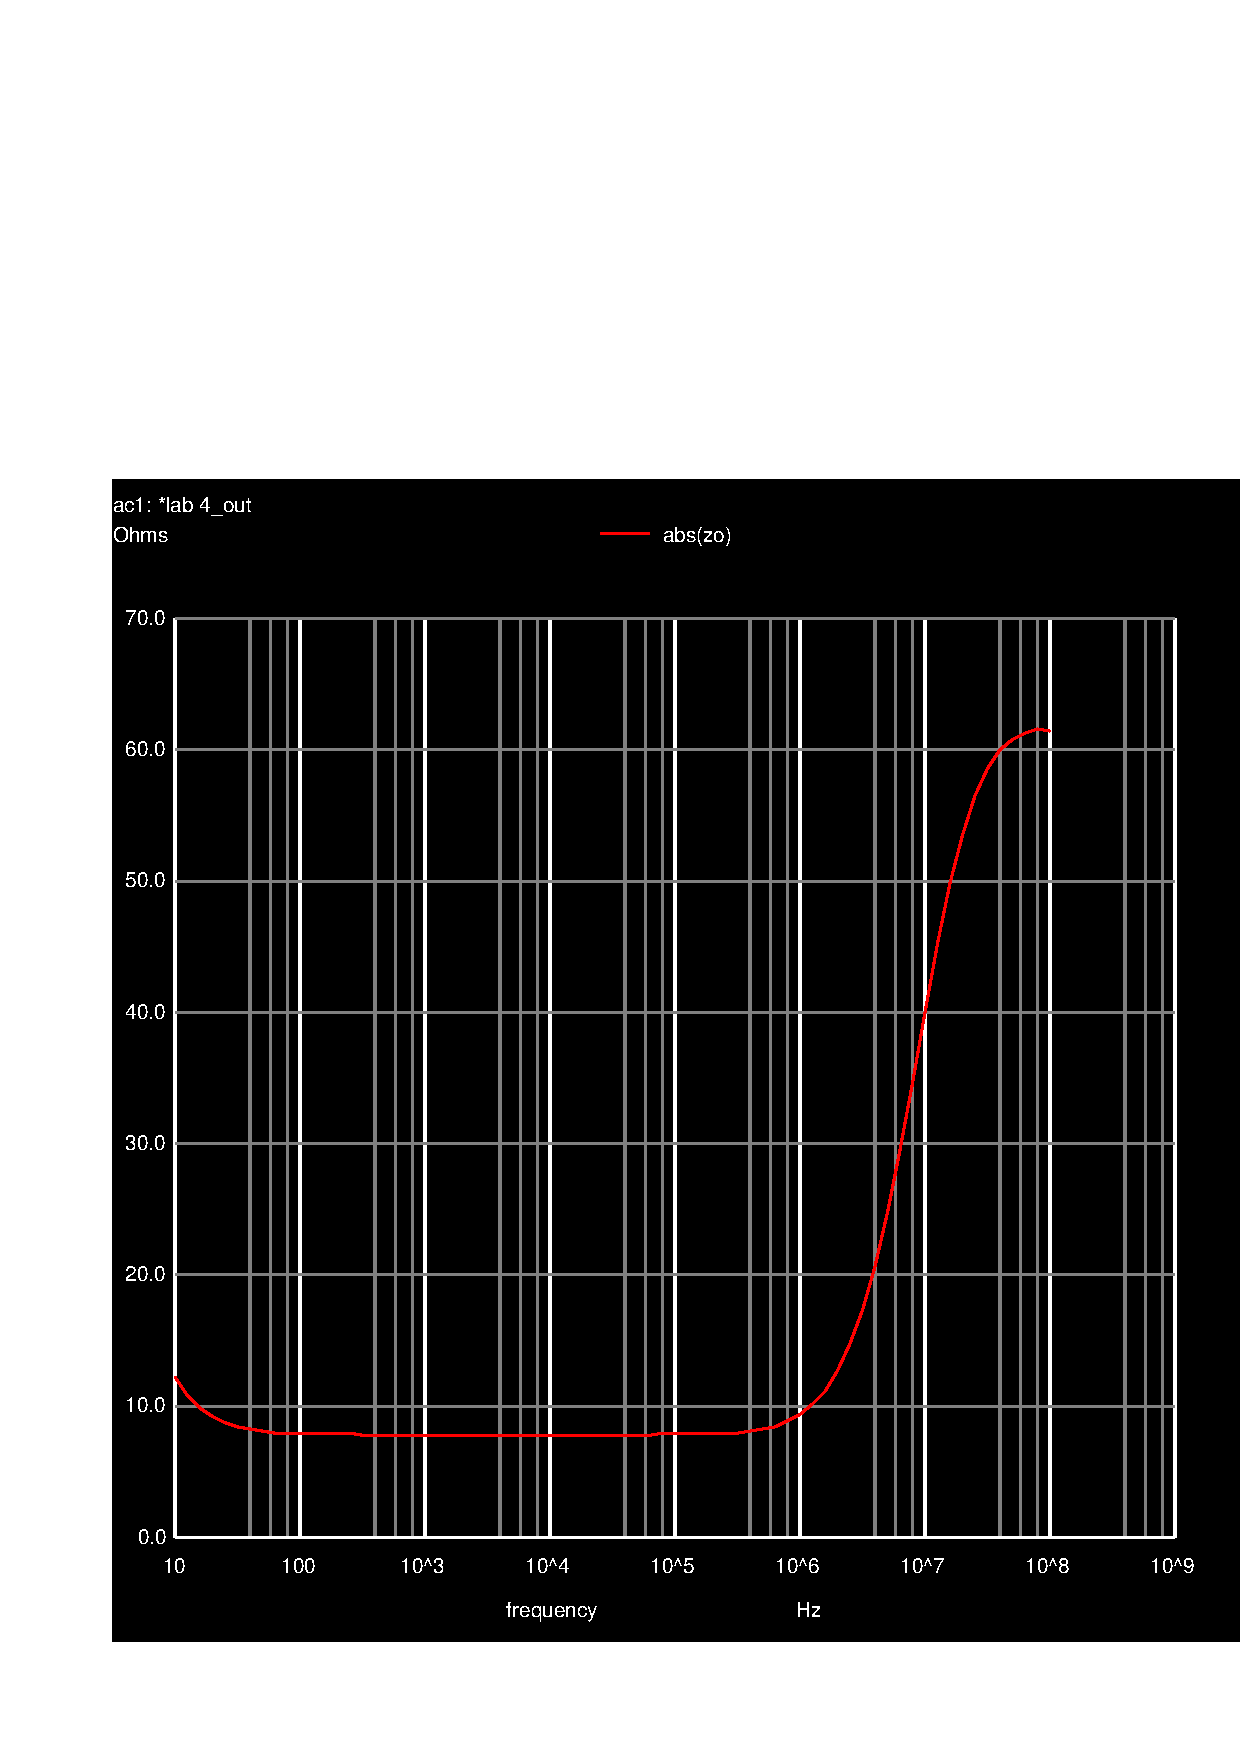
\includegraphics[width=7.5cm]{../sim/zout.pdf}
\caption{Frequency response of the output impedance of the circuit.}
\label{fig: output impedance}
\end{figure}



